% Analysing %
\chapter{Analysis of the Abstract Syntax Tree}
\label{chapter3}
The aim is to develop a model that can efficiently analyze the \astsmall created by \CLANG for our type of application. The \TOOL is based on this concept. In order to be able to make modifications to a program code, we first have to take a closer look at the \astsmall of the input application. The analysis will focus on identifying the different node classes provided by \CLANG and how they can be categorized for our use case. We also need to look at how the positions for the performance counters can be found in the representation and what further modifications are necessary to insert the counters at the correct location. Finally, we need to find out how the program flow can be structured and whether it is possible to develop a recursive model that can be applied to all classes.

\section{Identification of the Core Classes}
In \CLANG, all instructions are grouped into the superclasses \declssmall, \STATS, and types. The core classes, which contain definitions for \declssmall and \STATS, are particularly interesting for our field of application, since many basic functionalities of a program can be represented with the instructions described in these classes. We will not discuss subclasses of the core class types any further, since we do not require information about the data types of the instructions in our type of application. In the following the classes provided by the \CLANG framework must be grouped and it must be analyzed how they are handled by the \TOOL. 

The \declssmall class contains, among others, the classes \lstinline{FunctionDecl} and \lstinline{VarDecl}. These classes are used to represent descriptions of functions and variables in the \astsmall. Listing~\ref{lst:c:ast_declstmt_code} shows a code snippet of a program in which a main function is defined that contains assignments to different primitive data types of \CPP. The corresponding \astsmall representation of \CLANG is shown in Figure~\ref{fig:c:ast_declstmt}. The information contained in the \lstinline{FunctionDecl} class is needed to get the content of a function. In the \TOOL, this data is used to get the content of the main function at the beginning of the analysis process and to handle function calls. If we look at the \DECL of a variable in more detail, we notice that the variable \DECL itself is grouped under the \lstinline{DeclStmt} class. Since we do not need to distinguish between the different data types for the insertion of measurement code, it is sufficient to examine the higher-level class \lstinline{DeclStmt} more closely. This class, however, is located in the core class \STATS. This superclass also contains all the other classes that we need to specify more. In particular, we are interested in the classes


\begin{lstlisting}[float, language=C++, caption=Example Code Showing the Definition of Functions and Variables., label=lst:c:ast_declstmt_code]
int main(void) {
    int integer = 1;
    char character = 'a';
    bool boolean = true;
    float floatingPoint = 1.1;
    double doubleFloatingPoint = 1.2;
}
\end{lstlisting}

\begin{figure}[t]
    \centering
    \caption{The \AST for \DECLS of Functions and Variables.}
    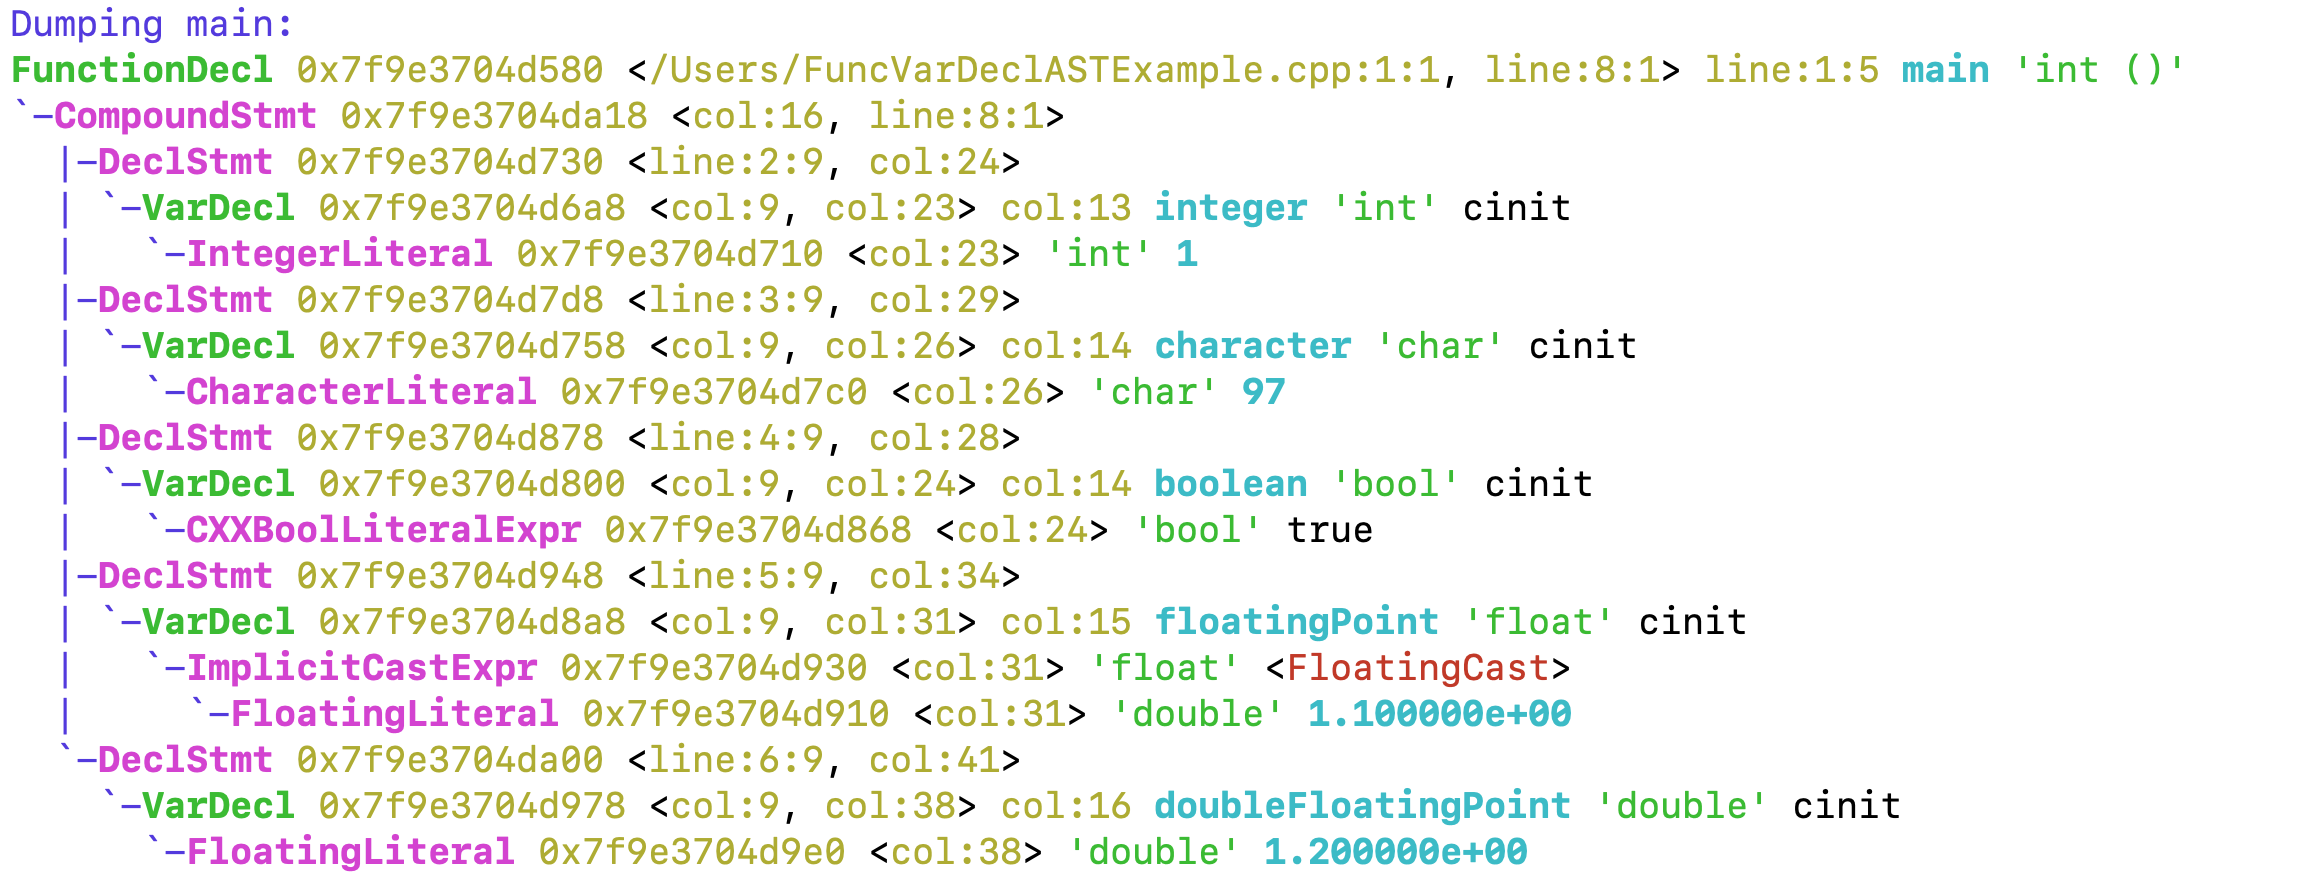
\includegraphics[width=1\textwidth]{graphics/c_ast_declstmt.png}
    \label{fig:c:ast_declstmt}
\end{figure}

\begin{itemize}[noitemsep, nolistsep]
    \item \lstinline{DeclStmt},
    \item \lstinline{OperatorCallExpr},
    \item \lstinline{BinaryOperator},
    \item \lstinline{CallExpr},
    \item \lstinline{CXXCallExpr},
    \item \lstinline{IfStmt},
    \item \lstinline{CaseStmt},
    \item \lstinline{ForStmt},
    \item \lstinline{DoStmt}, and
    \item \lstinline{WhileStmt}.
\end{itemize}

These classes were selected, since by describing these a variety of different programs can be analyzed by our transformation tool. These instructions provide basic functionalities which are used in each application and thus must be recognized by our profiler. We limit ourselves however in such a way that we do not have to identify each class which is made available by \CLANG, but address the most important classes mentioned before. 

\subsection{Leaf Nodes}
A group of \STATS is to be formed that contains operations that cannot be traversed further. We will call these instructions \LEASTAS. These include the frequently used classes \lstinline{DeclStmt}, \lstinline{OperatorCallExpr}, and \lstinline{BinaryOperator}. Nodes designated with the \lstinline{DeclStmt} class represent a variable \DECL. This operation can be neglected in the analysis of programs, since the runtime can be equated with a constant value. \lstinline{OperatorCallExpr} is used whenever an operator is called. For instance, this can occur when the software writes a value to a stream and outputs it. For nodes belonging to the \lstinline{BinaryOperator} class, two operands are used to get a result through a calculation or comparison. All three classes are examples of actions that are executed only once and cannot be further broken down into smaller parts. The group also contains other classes provided by the \CLANG framework that have similar characteristics. This group has the property that the \TOOL does not have to further traverse the instructions, but that measurement code can be directly be wrapped around them. 

\begin{lstlisting}[float, language=C++, caption=Example Code Showing the Definition of a Function Call., label=lst:c:ast_call_code]
void loopFunc() { 
    /* code block */ 
}

int main(void) {
    loopFunc();     // CallExpr Class
}
\end{lstlisting}

\begin{figure}[t]
    \centering
    \caption{The \AST for the \lstinline{CallExpr} Class.}
    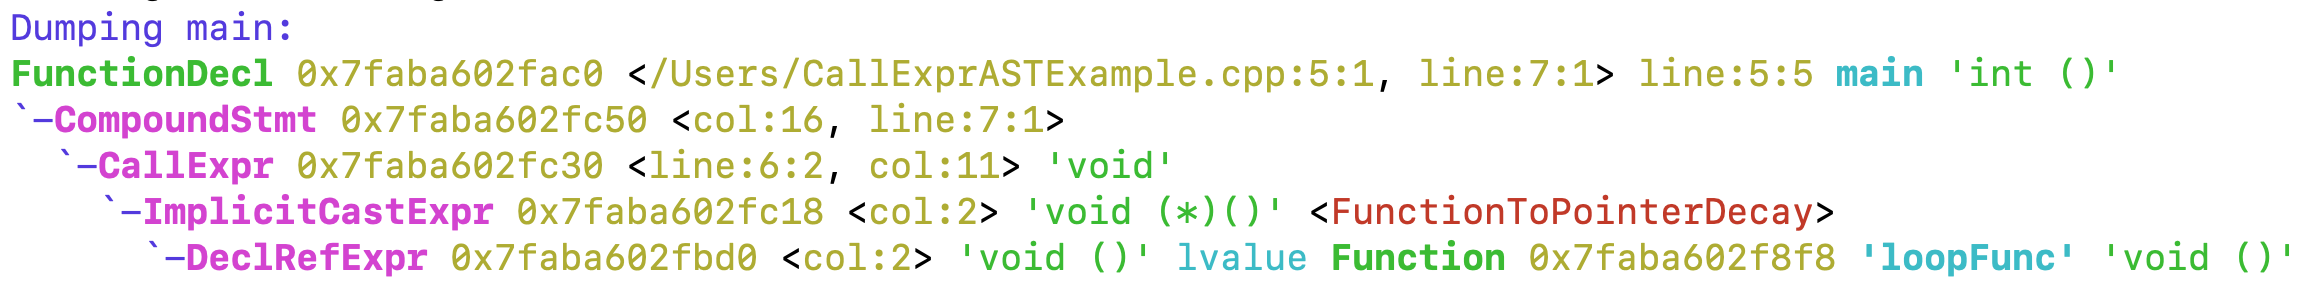
\includegraphics[width=\textwidth]{graphics/c_ast_call.png}
    \label{fig:c:ast_call}
\end{figure}

\subsection{Parent Nodes}
We will define all other classes in which we are interested in as \PARSTAS. These classes have the characteristics of an underlying layer that can also be traversed. They are of particular importance because we need to handle each special case of them separately. The code for a simple method call can be seen in Listing~\ref{lst:c:ast_call_code}. The corresponding representation in the \astsmall can be seen in Figure~\ref{fig:c:ast_call}, where the actual method call is specified by the class \lstinline{CallExpr}. In addition to the information about the location, this node also contains a reference to the function that is called. When the tool found this type of node it is necessary to check whether other nodes exist on the same level. If this is the case, the \PARSTA with all sub-levels can be enclosed as one unit with measurement code. If, however, there are no other siblings on this level, we must examine the subordinate level more closely. This is necessary because there would be no added value if only the runtime of a single possible resource-intensive class were output. In this case, we can use the \lstinline{getDirectCallee()} function provided by \CLANG to get the function that is called. For the class \lstinline{CXXMemberCallExpr} exactly the same approach can be applied.

\begin{lstlisting}[float, language=C++, caption=Example Code Showing the Definition of a Branch \STATLARGE., label=lst:c:ast_if_code]
int main(void) {
    int sum = 2;
    if(sum > 1)         { /* code block */ }
    else if(sum > 2)    { /* code block */ }
    else                { /* code block */ }
}
\end{lstlisting}

\begin{figure}[t]
    \centering
    \caption{The \AST for the \lstinline{IfStmt} Class.}
    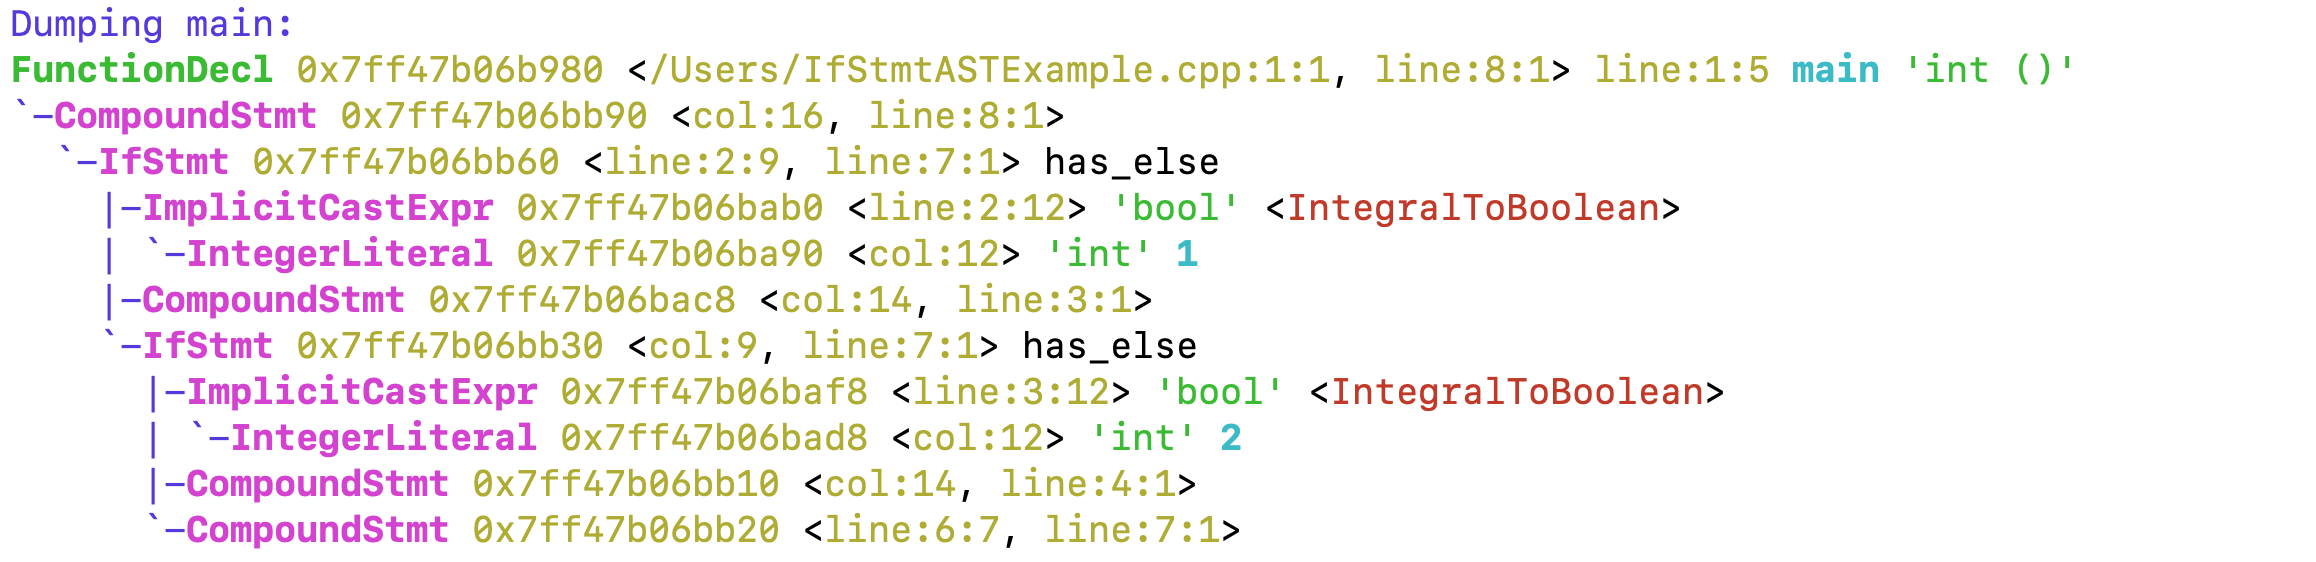
\includegraphics[width=\textwidth]{graphics/c_ast_if.png}
    \label{fig:c:ast_if}
\end{figure}

The code of a nested \lstinline{if-else}-query is shown in Listing~\ref{lst:c:ast_if_code}, with the associated \astsmall shown in Figure~\ref{fig:c:ast_if}. The first \lstinline{if}-\STAT represents the first query, whereas the nested \lstinline{if}-\STAT is actually an \lstinline{else-if}-branch. Both \lstinline{if}-\STATS have the \lstinline{has_else} flag, which means that there is an \lstinline{else}-branch in the query construction. To get the body of the \lstinline{if}-\STAT we use the \lstinline{getThen()} command. Once we have reached the last \lstinline{else-if}-branch, we check whether a flag labeled \lstinline{has_else} is set and in this case we can execute a \lstinline{getElse()} query. Nodes belonging to the Class \lstinline{CaseStmt} can be traversed analogously to \lstinline{if}-\STATS with the same method, but instead of the \lstinline{getThen()} function we use the \lstinline{getBody()} function.

\begin{lstlisting}[float, language=C++, caption=Example Code Showing the Definition of a Loop., label=lst:c:ast_for_code]
int main(void) {
    for(int i = 0; i < 10; i++) { /* code loop */ }
}
\end{lstlisting}

\begin{figure}[t]
    \centering
    \caption{The \AST for the \lstinline{ForStmt} Class.}
    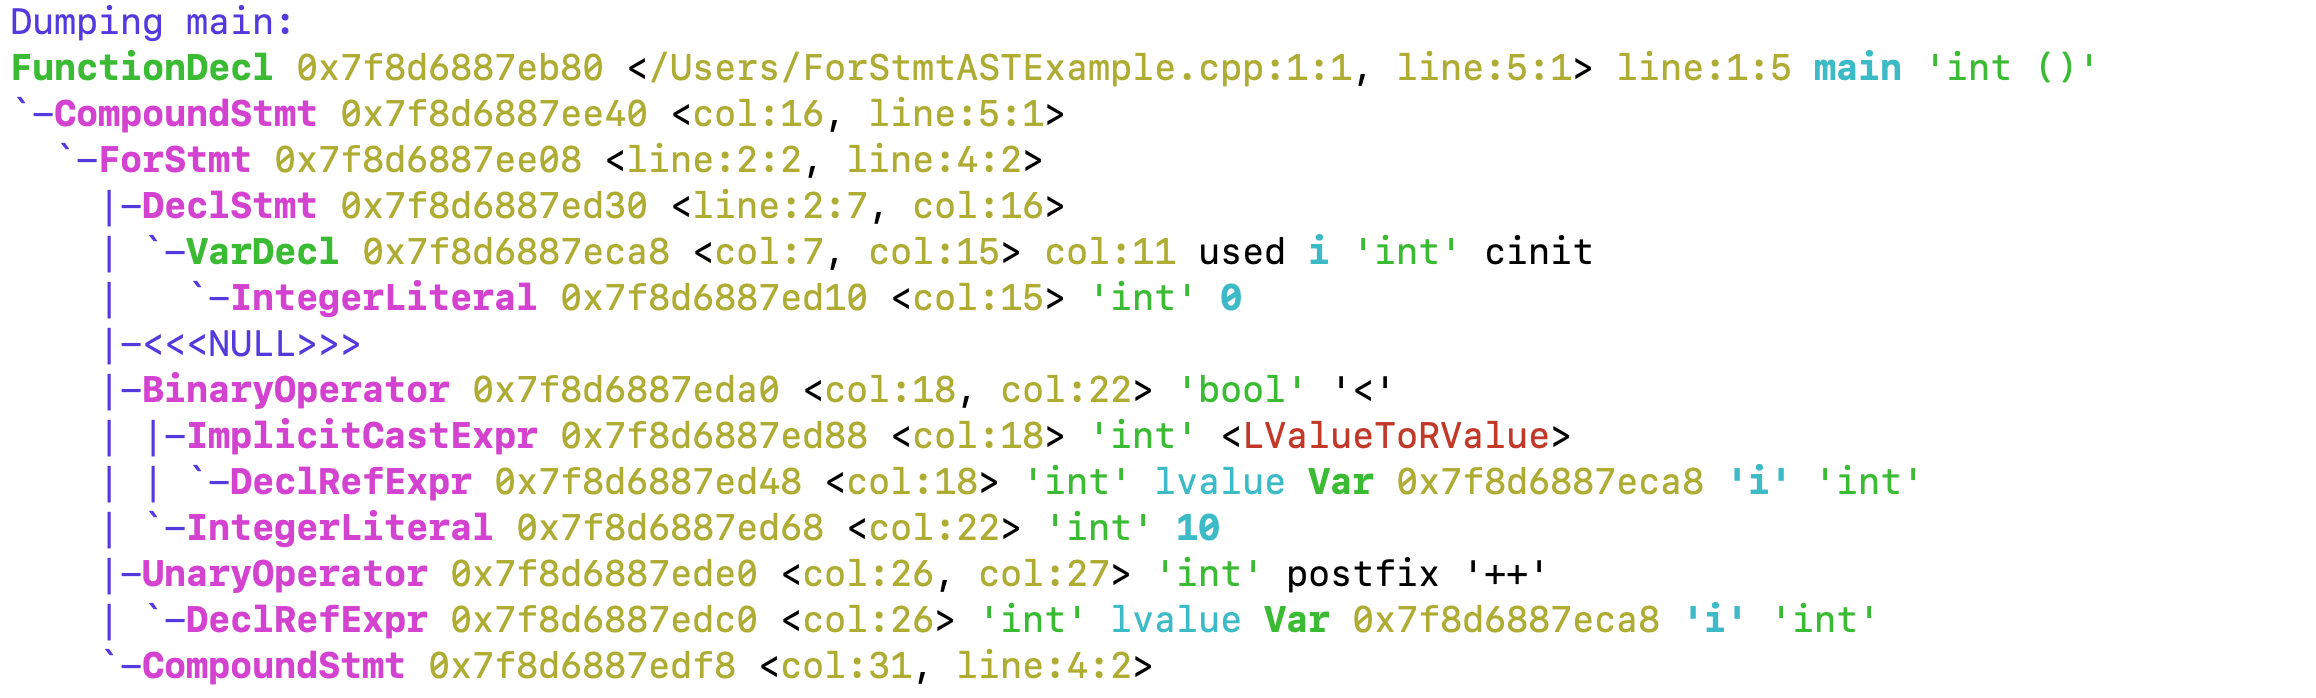
\includegraphics[width=\textwidth]{graphics/c_ast_for.png}
    \label{fig:c:ast_for}
\end{figure}

The implementation of a \lstinline{for}-loop, another \PARSTA that needs to be analyzed, can be seen in Listing~\ref{lst:c:ast_for_code}. The \astsmall generated from the code can be seen in Figure~\ref{fig:c:ast_for}. The analysis of loops is particularly complicated because the instructions in them can be executed several times. To get the content of the loop, we can simply use the function \lstinline{getBody()}, but the runtime calculation of the performance counter inserted there has to be taken into account. This is problematic because the inserted measurement code is called as often as the loop itself. The times of individual instructions must therefore be added together so that the total time of a \STAT can be calculated. The problem of the overhead generation will be discussed in more detail in Chapter~\ref{chapter5}. The process of traversing \lstinline{while}- and \lstinline{do/while}-loops can be treated analogously to that of \lstinline{for}-loops. It can thus be stated that \PARSTAS are only enclosed with performance counters if other elements exist on the same level. If this is not the case, the tool can immediately analyze the underlying level.

Furthermore, the \asts in Figure~\ref{fig:c:ast_call}, Figure~\ref{fig:c:ast_if}, and Figure~\ref{fig:c:ast_for} show nodes with the label \lstinline{CompoundStmt}. This is used to group children of a superordinate node. In the \lstinline{CompoundStmt} provided by \CLANG, however, there are nodes from both of the groups we identified. Instructions that belong to the group of \LEASTAS, including simple \declssmall of variables, should also be grouped together. To do this, however, classes that themselves contain further children must be removed and treated separately. For this purpose, we will create a separate class called \lstinline{CustomCompoundStmt} when traversing. For each node traversed, the tool checks which group it belongs to. If the current node is a \LEASTA, it is added to a \lstinline{CustomCompoundStmt} or a new \lstinline{CustomCompoundStmt} is initialized. A node of type \lstinline{CustomCompoundStmt} is closed when the first \PARSTA is reached. After this class has been handled separately, a new \lstinline{CustomCompoundStmt} can be initialized. This allows the runtime of all \LEASTAS to be combined. It should also be mentioned that this grouping is not done at runtime of the input program, but already in the analysis process of the tool, which reduces the resource consumption of the tool. 

\begin{lstlisting}[float, language=C++, caption=Fibonacci Application Example for Analysing the Identified Groups., label=lst:c:example_categorisation]
#include <iostream>

int fibonacci() {
    /* CustomCompoundStmt start */
    double n = 0;                               // leaf node
    t1 = 0;                                     // leaf node
    t2 = 1;                                     // leaf node
    nextTerm = 0;                               // leaf node
    n = 100;                                    // leaf node
    std::cout << "Fibonacci Series: ";          // leaf node
    /* CustomCompoundStmt end */

    for (int i = 1; i <= n; ++i) {              // parent node
        if(i == 1) {                            // parent node
            /* CustomCompoundStmt start */
            std::cout << t1;                    // leaf node
            std::cout << ", ";                  // leaf node
            /* CustomCompoundStmt end */
        }
        else if(i == 2) {                       // parent node
            /* CustomCompoundStmt start */
            std::cout << t2;                    // leaf node
            std::cout << ", ";                  // leaf node
            /* CustomCompoundStmt end */
        }
        /* CustomCompoundStmt begin */
        nextTerm = t1 + t2;                     // leaf node
        t1 = t2;                                // leaf node
        t2 = nextTerm;                          // leaf node
        std::cout << nextTerm << ", ";          // leaf node
        /* CustomCompoundStmt end */
    }
}

int main(void) {
    fibonacci();                                // parent node
    return 0;
}
\end{lstlisting}

\subsection{Classification Approach by Example}
The collected knowledge about the classes of the nodes can now be used to analyze the example code, shown in Listing~\ref{lst:c:example_categorisation}, of an application that calculates the first hundred Fibonacci numbers. In order to better understand the procedure of the \TOOL, we will also start traversing the nodes in the main function. In the first line of the main function, a function call can be seen, which can be classified as a \PARSTA, since the sub-tree of the function \DECL can be accessed by calling this function. In the first sub-level of the function \DECL, there are first six instructions that can be marked as \LEASTAS, since no further levels can be reached through these nodes. Furthermore, these instructions can be combined as \lstinline{CustomCompoundStmt}, as the individual runtimes will be negligible. Next, there is a \lstinline{for}-loop that must be declared as a \PARSTA, since further instructions are called from it. The two \lstinline{if}-instructions found in the level below also contain children and are therefore also defined as \PARSTAS. Each instruction contains two simple instructions that can declared as \LEASTA and grouped together as \lstinline{CustomCompoundStmt}. At the end of the function there are four more instructions that are also marked as \LEASTAS and can be combined. It should be noted that in the actual traversal process not all levels are annotated at once. If the \TOOL is executed without further options, only the content of the \lstinline{fibonacci()} function would be annotated for the time being. With the information gained from the first run, the user can specify a desired region to be looked at in more detail. 

Finally, it can be stated that the nodes of the \astsmall can be divided into two groups for our purposes. \emph{Leaf nodes} that are summarized as \lstinline{CustomCompoundStmt} and \PARSTAS that have to be considered separately. For groups of \LEASTAS, only one shared runtime is calculated by the \TOOL. \emph{Parent nodes} are tracked individually if other instructions exist on the same level. If only one superclass is found on the currently examined level, its content is analyzed in more detail. If the special case occurs that each level contains only one instruction, only the total runtime of the program is calculated and output, as no detailed profiling statistic can be provided for the input application. 

\section{Detection of the Insert Locations}
In order to insert the measurement code in the right places, we need information about the positions of the nodes in the actual program code. These are stored in the \SOUMNG of the \astsmall and can be accessed by calling functions of the \CLANG infrastructure. For the \TOOL, functions that access the first and last location of the node are particularly important. However, the results of these predefined functions must be modified. If we now use the functions to obtain the boundary positions of a node and insert our measurement code into them, we get an output that looks similar to the code shown in Listing~\ref{lst:c:insertion_lexer}. It can be seen that the example code was inserted correctly before the instruction under consideration, but the end tag differs from the desired result. To generate code that creates the desired result, the code must be inserted after the closing curly brace. However, the locations obtained with the \lstinline{getBeginLoc()} function can be used immediately to insert the code at these locations. 

\begin{lstlisting}[float, language=C++, caption=Wrong Insertion Position When Using End Location of Node., label=lst:c:insertion_lexer]
void loopFunc() {
    startEvent(1);          // getBeginLoc() returns the correct position
    while ( i <= 10 ) { 
        i++; 
        endEvent(1);        // getEndLoc() returns the incorrect position
    }
    /* "endEvent(1);" should be inserted at the position after the brace */
}
int main(void) {
    startEvent(0);
    loopFunc();
    endEvent(0);
    print();
    return 0;
}
\end{lstlisting}

The function \lstinline{getEndLoc()}, on the other hand, does not return the first place after the examined node, but the last place in it. As can be seen in Listing~\ref{lst:c:insertion_lexer}, this leads to the measurement code not correctly enclosing the node. If the instruction does not contain opening and closing brackets, the position before the semicolon may also be returned. Both problems can be solved analogously. The solution is to develop a function that checks the current token and moves the position with the information obtained. To do this, first check whether the token at the current position is of type \lstinline{clang::tok::semi} or of type \lstinline{clang::tok::r_brace}, which allows the parameters for subsequent actions to be determined. Afterwards, the interface \emph{Lexer} provided by \CLANG, which allows certain actions on the streams of tokens, can be used to find the desired position with the function \lstinline{Lexer::FindLocationAfterToken()}. This method takes the current token and the character to be searched for and returns the position after the first character searched for. Finally, we can state that the start position and the end position of all nodes are now returned correctly for our purposes. With these positions, the measurement code can be wrapped around different groups of nodes. 

\section{Application of a Recursive Model to the Core Classes}
\begin{figure}[p]
    \centering
    \caption{Flow Chart Representing the Logic of the \TOOL.} 
    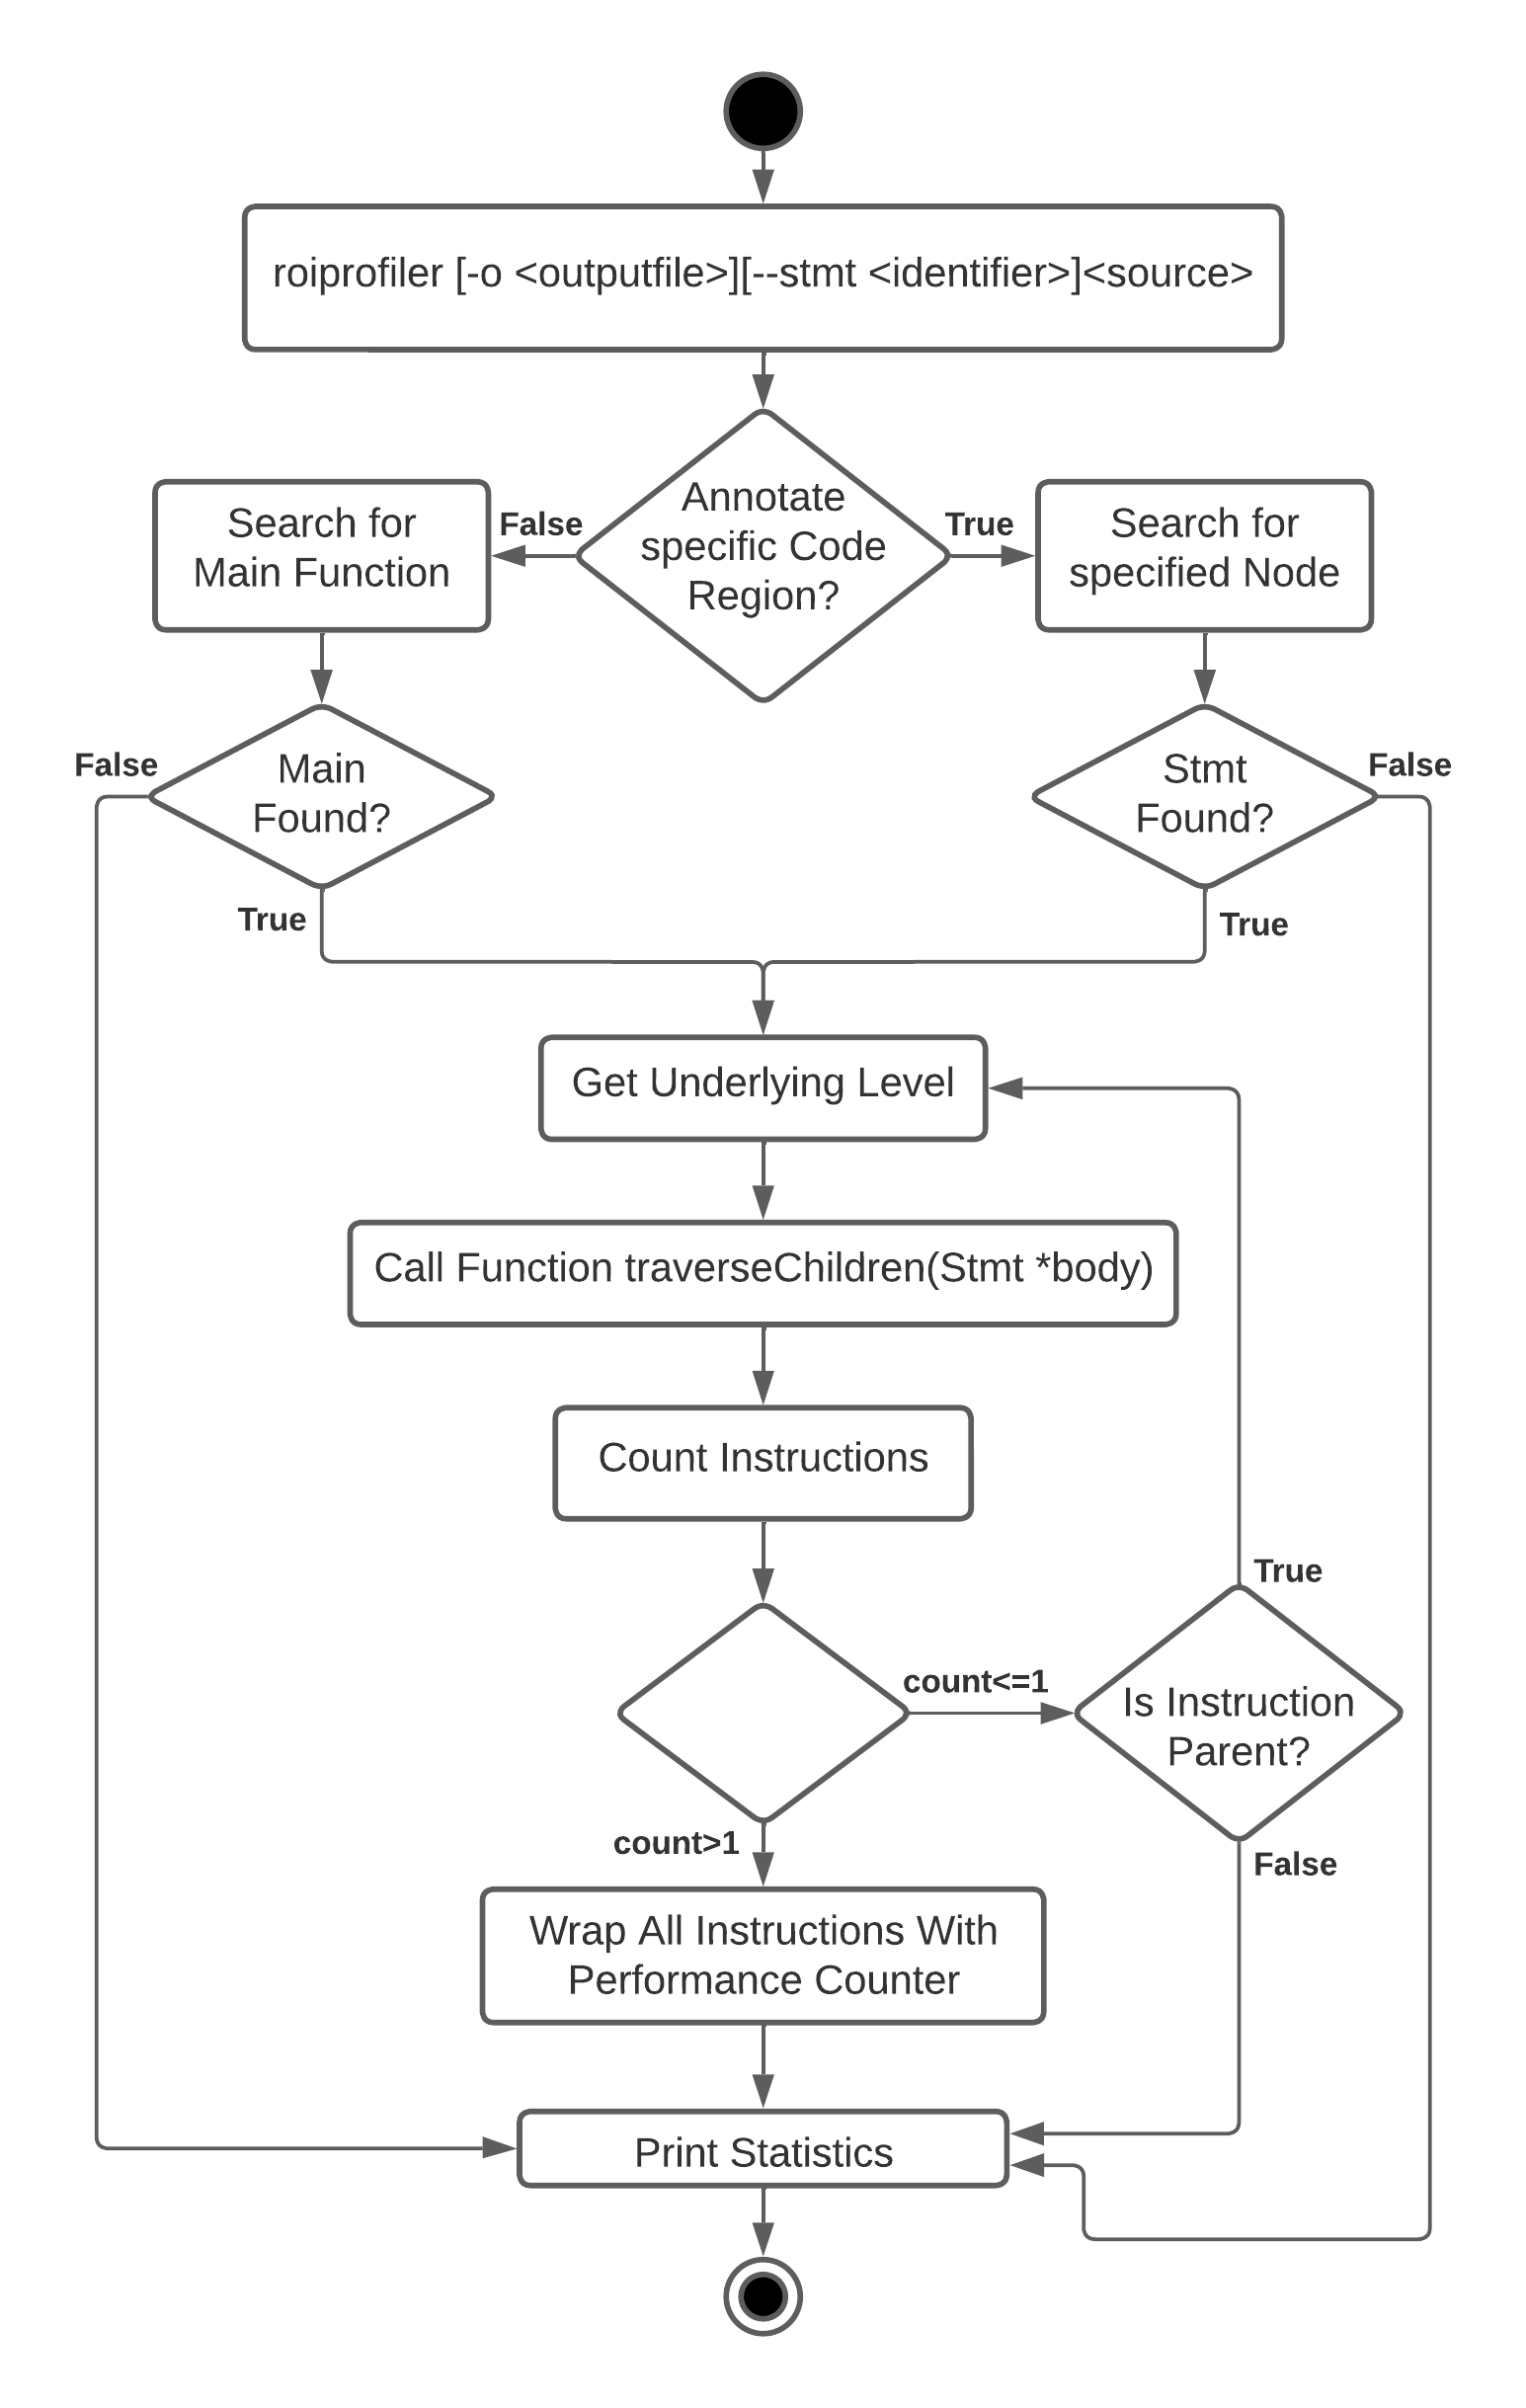
\includegraphics[width=.75\textwidth]{graphics/c_flow_chart.png}
    \label{fig:c:flow_chart}
\end{figure}

In the following we discuss the flow of the \TOOL and explain how all the different types of nodes can be traversed recursively. For this purpose, the input parameters and the expected output of the \TOOL should be defined first. As a mandatory input parameter, the \TOOL should accept a source code written in \C /\CPP. The storage location for the transformed program can be specified optionally. Furthermore, the user can decide in which \roismall instructions are to be annotated. At the beginning of the profiling process, the \TOOL should wrap all code blocks of the main function with performance counters and return transformed software that can be executed by the user. In addition to the actual output of the input program, the user is provided with useful feedback on the resource consumption of individual instructions in the main function. Each instruction that supports a more detailed analysis is shown with an identification number. The user can utilize these identifiers to start the next iteration of the analysis by specifying desired regions and launching the \TOOL again. 

Now that the basic characteristics of our tool are known, the logic of the process behind it can be analyzed. A flow diagram of the simplified process is shown in Figure~\ref{fig:c:flow_chart}. The process is started by calling the \TOOL with the correct parameters. The first step is to check which mode is currently active and, depending on this, either search for the \ENTPOI to the input application or search for an instruction specified by the user. In both cases, the source code created by \CLANG is first searched for the desired node. The \TOOL is terminated if neither a main function nor a node with the searched identifier is found. If the search is successful, the node found of the instruction is passed to the \lstinline{traverseChildren(Stmt*)} function. Further, the content of the passed node is taken so that the child nodes can be counted and categorized. The number of children is needed to make a basic case distinction. If several nodes are located at this level, they can be annotated and the program can be terminated. However, if only one node is found at this level, it must be checked whether it belongs to the group of \PARSTAS. The special case of only one instruction occurring in each level is achieved if the node is not a \PARSTA. In this case, only the runtime of the entire application is returned, as no analysis of individual instructions is possible. However, if the \TOOL detects another level that can be analyzed, the content of the \PARSTA can simply be forwarded recursively. 

In the process shown in Figure~\ref{fig:c:flow_chart}, it can be stated that all properties for the development of a recursive method apply. In general, the overarching problem is to examine all levels of the \astsmall and to assign performance counters to certain sub-areas. The sub-problem is to examine a single level of the tree and to examine nodes on this level. Furthermore, the \TOOL has two base cases that serve as termination conditions. One is met when multiple nodes at a level are found, in which case we can simply annotate them all and solve the problem. The other termination condition is given if only one \LEASTA exists which has no other levels below it. If there is only one instruction on a level that has other child nodes, we can simply traverse that level by calling the function itself. This procedure is repeated until either all levels have been traversed, or until a level has been found that can be annotated and the overall problem has been solved. This is very useful, since it is not necessary to consider each level separately, or even to count the depth of the \astsmall at the beginning. Thus, it makes no difference how many levels are below the starting point, as the program only terminates after the last level has been reached. 

\subsection{Traversing Approach by Example}
Based on this method, the example code shown in Listing~\ref{lst:c:example_traverse} can now be analyzed. When the traversal process begins, the main function is searched for and checked to see how many instructions have been specified in it. In this case, the main function contains only one instruction of the type \lstinline{CallExpr} (\lstinline{loopFunc()}). Since a node was found that has subordinate levels, the contents of this can be passed on to the \lstinline{traverseChildren(Stmt*)} function. Subsequently, the children of this node are also examined, but this time an instruction of the class \lstinline{ForStmt} is present. This class also falls into the group of \PARSTAS and the content must therefore be traversed again. On the next level, it is noticeable that not only one \LEASTA is to be executed. The termination condition is reached and all nodes on this level can be wrapped with performance counters. If we change the example a little and give the tool the identifier of the \lstinline{for}-loop in the \lstinline{loopFunc()} function as the starting point, all previous steps would be skipped by the \TOOL and the body of the \lstinline{for}-loop can be annotated immediately. With the insertion of the performance counters, the first run of the profiling process is finished, and the user now has the option of running the \TOOL again with the identifiers of the \lstinline{while}-loops to start a more detailed analysis of them.

\begin{lstlisting}[float, language=C++, caption=Example of the Model Used to Traverse the \AST., label=lst:c:example_traverse]
void loopFunc() {
    // children.size() <= 1 && child.getClass() == Stmt::ForStmtClass
    // // => traverseChildren(child.getBody())
    for (int i = 0; i < 10; i++) {
        // children.size() > 1 
        // => annotate all instructions
        for { /* code loop 1 */ }
        for { /* code loop 2 */ }
        for { /* code loop 3 */ }
    }
}

int main(void) {
    // children.size() <= 1 && child.getClass() == Stmt::CallExpr
    // => traverseChildren(child.getBody())
    loopFunc();                                            
}
\end{lstlisting} 

Finally, it can be stated that a model was found with which all classes of the group of \PARSTAS can be treated equally. After the categorization of the nodes, depending on the class type, it can be determined how the underlying \lstinline{CompoundStmt} class can be accessed. If access is gained to this node, it can be passed on as a node of the superclass \lstinline{Stmt} as a parameter to the \lstinline{traverseChildren(Stmt*)} function. The fact that the node can be represented as a \lstinline{Stmt} is particularly important, as all the functions necessary for our purpose can be accessed. From this point on, the procedure is the same for all classes. It can therefore be said that when applying this model, it makes no difference which type of \PARSTA is to be traversed. This is very useful, as a single recursively defined function is sufficient to traverse the sub-levels of all class types.
